\documentclass[a4, danish]{article}

\usepackage{import} 
\import{../../LaTeX-Preamble/}{preamble_dk.tex}

\settitle{Dispositioner}{Regularitet og Automater}
\addauth{Martin Nørskov Jensen}{201610882@post.au.dk}{au553262}

\begin{document}

\maketitle
\newpage    
\tableofcontents

\newpage
\section{Regulære udtryk}
  \subsection{Regulære sprog}
  \begin{itemize}
    \item Et sprog S er et regulært sprog, hvis det kan beskrives af et regulært udtryk
    \item Sproget L(r) over et regulært udtryk er defineret i strukturen af r, således: 
    \begin{itemize}
      \item $L(\emptyset)=\emptyset $
      \item $L(\Lambda)=\{ \Lambda \}$
      \item $L(a)=\{a\}$
      \item $L(r_1+r_2)=L(r_1)\cup L(r_2)$
      \item $L(r_1r_2)=L(r_1)L(r_2)$
      \item $L(r_1^*)=L(r_1)^*$
    \end{itemize}
    \item $L(\emptyset^*)=L(\Lambda)$ så $\Lambda$ kan betragtes, som en forkortelse af $\emptyset^*$
    \item Operationer på regulære sprog
    \begin{itemize}
	    \item Foreningsoperation: givet to sprog $L_1,L_2\subseteq \Sigma^*$, så er forening af de to sprog defineret ved:
      \begin{equation*}
        L_1\cup L_2 = \{x \ | \ x\in L_1 \lor x\in L_2 \}
      \end{equation*}
      \item Konkateneringsoperation: givet to sprog $L_1,L_2\subseteq \Sigma^*$, så er konkateneringen af de to sprog defineret ved:
      \begin{equation*}
        L_1L_2= \{xy \ | \ x\in L_1 \land y\in L_2 \}
       \end{equation*}
      \item Kleenesstjerneoperation: givet et sprog $L \subseteq \Sigma^*$, så er Kleene stjerne af det sprog defineret ved:
      \begin{align*}
        L^* &= \bigcup_{i=0}^{\infty} L^i \\
            &= L^0\cup L^1 \cup L^2 \cup L^3  \\
            &= \{\Lambda \} \cup L \cup LL \cup LLL 
      \end{align*}
    \end{itemize}
    \item Klasser af formelle sprog:
    \begin{figure}[ht!]
	  \centering
	  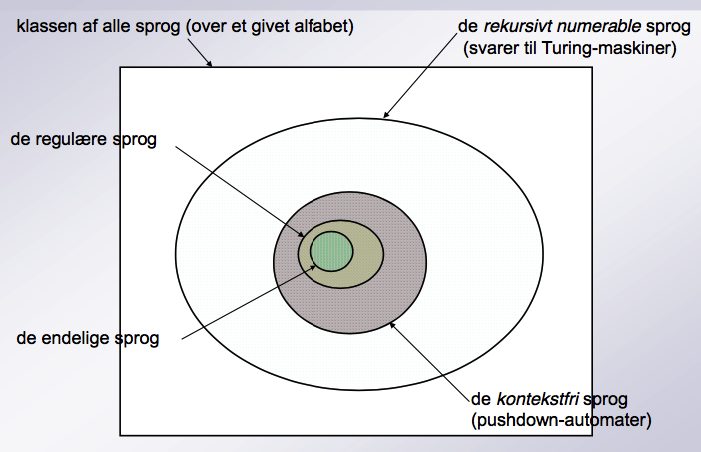
\includegraphics[width=70mm]{img/sprogklasser.png}
	  \caption{Klasser af formelle sprog	\label{formelleSprog}}
  \end{figure}
  \end{itemize}
  \subsection{Endelige automater}
  \begin{itemize}
    \item En FA accepterer et regulært sprog, hvorimod et regulært udtryk beskriver det
    \begin{itemize}
      \item En FA og et regulært udtryk har samme udtrykskraft, det vil sige, at de kan beskrive den samme mængde sprog. 
      \item Givet en streng svarer den enten ja eller nej 
    \end{itemize}
    \item Eksempel på en endelig automat over alphabet $\Sigma=\{0,1\}$, der accepterer en streng med et lige antal 0'er
    \begin{figure}[ht!]
	  \centering
	  \includegraphics[width=60mm]{img/FAeks.png}
	  \caption{Eksempel på en endelig automat	\label{FAeks1}}
    \end{figure}
    \item En finite automat er en 5-tuple $(Q, \Sigma, q_0, A, \delta)$
    \begin{itemize}
	    \item $Q$ er et endeligt mængde tilstande
      \item $\Sigma$ er et alfabet
      \item $q_0 \in Q$ er start-tilstanden
      \item $A \subseteq Q$ er endelig mængden af accept tilstande
      \item $\delta: Q \times \Sigma \rightarrow Q$ er transitionsfunktionen, som givet en tilstand og et tegn returnerer en tilstand. 
    \end{itemize}
    \item Den udvidet transitionsfunktion: $\delta^*: Q \times \Sigma^* \rightarrow Q$ er defineret på følgende måde for alle $q\in Q$ og $x \in \Sigma^*$
 	 	\begin{equation*}
		\delta^*(q,x) =
		\begin{cases}
			\mbox{$q$} & \mbox{hvis $x = \Lambda$} \\
			\mbox{$\delta(\delta^*(q,y),\sigma)$} & \mbox{hvis $x=y\sigma$ for alle $\sigma \in \Sigma$ og $y\in \Sigma^*$} \\
		\end{cases}
		\end{equation*}
    \item Sproget for en endelig automat M er defineret på følgende måde:
    \begin{equation*}
      L(M)=\{x \in \Sigma^* \ | \ \delta^*(q_0,x)\in A \}
    \end{equation*}
    \item Kleenes sætning siger: \textit{"For et hvert alphabet $\Sigma$, ethvert regulært sprog kan blive accepteret af en FA"}
    \begin{itemize}
    	\item Dette kan vises ved brug NFA'er, som et konstruktivt induktionsbevis i strukturen af de regulære udtryk.
      \item NFA'er kan repræsentere, den samme mængde sprog, som FAer og NFA og dette kan man vise, ved hjælp af følgende 
    \end{itemize}
  \end{itemize}
  \begin{figure}[ht!]
  	  \centering
  	  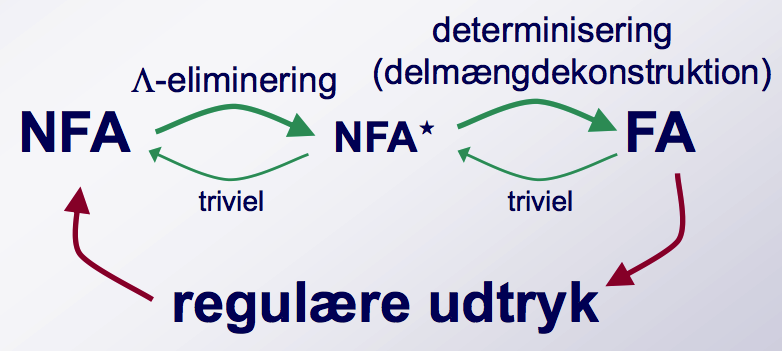
\includegraphics[width=100mm]{img/automater}
  	  \caption{Konversion mellem forskellige automater	\label{automater1}}
    \end{figure}
   \subsection{Bevis for kleenes sætning del. 1}
    \textbf{Basis:}\\
    $r=\emptyset$: \\
    Hvis det regulære udtryk er det tomme regulære udtryk, sætter vi vores automat, til at være den pågældende automat: \\
    \begin{figure}[h]
    	  \centering
    	  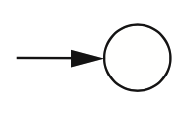
\includegraphics[width=25mm]{img/Kleene11.png}
    	  \caption{Automaten for sproget $L(\emptyset)$	\label{KleeneBasis1}}
    \end{figure}
    \\
    $r=\sigma$:\\
    Hvis det regulære udtryk er tegnet $\sigma$ sætter vi vores automat til at være den pågældende automat:
    \begin{figure}[ht!]
  	  \centering
      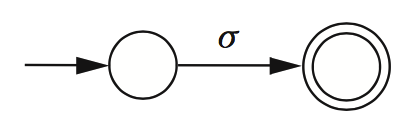
\includegraphics[width=50mm]{img/Kleene12.png}
  	  \caption{Automaten for sproget $L(\sigma)$	\label{KleeneBasis2}}
    \end{figure}
    \\
    \textbf{Induktionskridtet:} \\
    Vores induktionen hypotese er, at der findes en NFA $M_i=(Q_i,\Sigma,q_i,A_i,\delta_i)$ der accepterer vores sammensatte udtryk $L(r_i)$ \\
    $r=r_1+r_2$: \\
    Vi har fra vores induktionshypotese, at der findes to automater, som accepterer sproget $L(r_1)$ og sproget $L(r_2)$ sætter vi automat til at være
    \begin{align*}
      M_r&=(Q_r,\Sigma,q_r,A_r,\delta_r) \\
      Q_r&=Q_1\cup Q_2 \cup \{q_r\} \\
      A_r&=A_1\cup A_2 
    \end{align*}
    Vi sætter vores transitionsfunktionen til at være 
    \begin{equation*}
		  \delta_r(q,x) =
  		\begin{cases}
  			\mbox{$\delta_1(q,x)$} & \mbox{hvis $q\in Q_1$} \\
  			\mbox{$\delta_2(q,x)$} & \mbox{hvis $q\in Q_2$} \\
   			\mbox{$\{q_1, q_2\}$} & \mbox{hvis $q=q_r$  og $x=\Lambda$} \\
  		\end{cases}
		\end{equation*}
    og tilføjer transitioner ud fra vores starttilstand $q_r$, som tillader os at bevæge os både ind i  $q_1$ og $q_2$
    \begin{equation*}
      \delta_r(q_r,\Lambda)=\{q_1,q_2\}
    \end{equation*}
    Vi får dermed følgende automat, som accepterer sproget $L(r_1)\cup L(r_2)$:
    \begin{figure}[ht!]
  	  \centering
  	  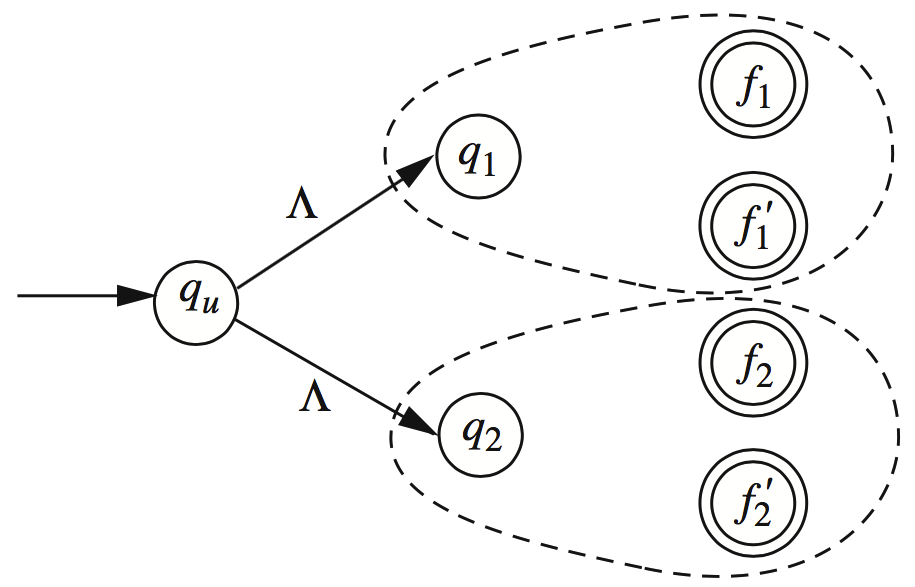
\includegraphics[width=80mm]{img/Kleene13.png}
  	  \caption{Automaten for sproget $L(r_1)\cup L(r_2)$	\label{KleeneInd1}}
    \end{figure}
    \\
    Bevis for at $x \in L(r) \Leftrightarrow x \in L(M_r)$:
    \begin{itemize}
    	\item  $x \in L(r) \Rightarrow x \in L(M_r) $: 
      \begin{align*}
        x \in L(r) = L(r_1+r_2) \\
        \Rightarrow x \in L(r_1) \cup L(r_2) \\
        \Rightarrow x \in L(r_1) \lor L(r_2) 
      \end{align*}
      Bliver altid accepteret af $M_r$, da der findes en sti til accepttilstande, som acceptere $L(r_1)$ og $L(r_2)$       
      \item  $x \in L(r) \Leftarrow x \in L(M_r) $: 
      \begin{align*}
        x \notin L(r) &\Rightarrow x \notin L(M_r) \\
        x \notin L(r) &\Rightarrow x \notin L(r_1) \land x \notin L(r_2) \\
        &\Rightarrow x \notin L(M_r)
      \end{align*}
    \end{itemize}
    $r=r_1r_2$:\\
    Vi sætter her vores NFA til at være 
    \begin{align*}
      M_r&=(Q_r,\Sigma,q_1,A_2,\delta_r)\\
      Q_r&=Q_1\cup Q_2 
    \end{align*}
    Vi sætter så vores transitionsfunktion til at være:
    \begin{equation*}
		  \delta_r(q,x) =
  		\begin{cases}
  			\mbox{$\delta_1(q,x)$} & \mbox{hvis $q\in Q_1$} \\
  			\mbox{$\delta_2(q,x)$} & \mbox{hvis $q\in Q_2$} \\
        \mbox{$\{q_2\}$} & \mbox{hvis $q\in A_1$ og $x=\Lambda$} \\
  		\end{cases}
		\end{equation*} 
    Hermed få vi følgende automat, som accepterer sproget $L(r_1)L(r_2)$:
    \begin{figure}[ht!]
  	  \centering
  	  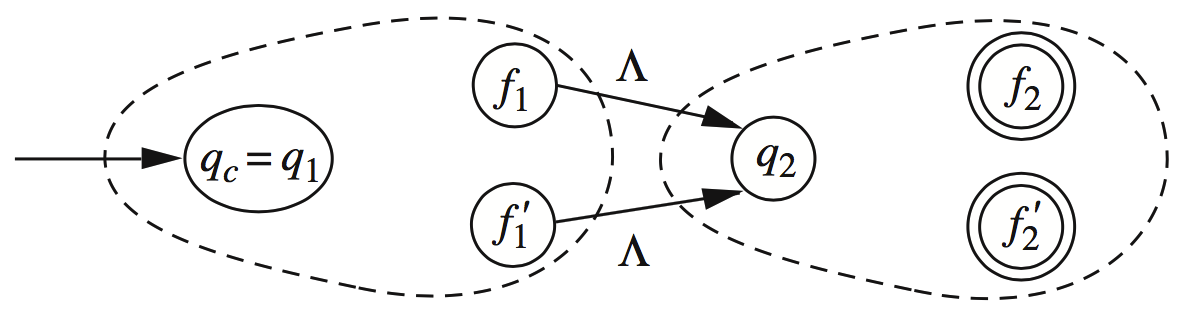
\includegraphics[width=100mm]{img/Kleene14.png}
  	  \caption{Automaten for sproget $L(r_1)L(r_2)$	\label{KleeneInd2}}
    \end{figure}
    \\
    $r=r_1^*$:\\
    Vi sætter her vores NFA til at være:
    \begin{equation*}
      M_r=(Q_1\cup \{q_0\},\Sigma,q_0,\{q_0\},\delta_r)\\
    \end{equation*}
    Vi sætter vores transitionsfunktion til at være følgende:
        \begin{equation*}
		  \delta_r(q,x) =
  		\begin{cases}
  			\mbox{$\delta_1(q,x)$} & \mbox{hvis $q\in Q_1$} \\
        \mbox{$\{q_0\}$} & \mbox{hvis $q\in A_1$ og $x=\Lambda$} \\
        \mbox{$\{q_1\}$} & \mbox{hvis $q=q_0$ og $x=\Lambda$} \\
  		\end{cases}
		\end{equation*} 
    \begin{figure}[ht!]
  	  \centering
  	  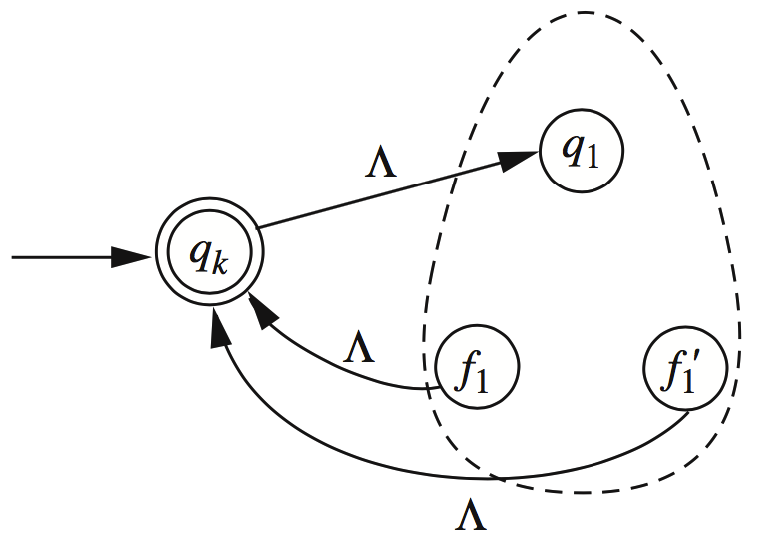
\includegraphics[width=80mm]{img/Kleene15.png}
  	  \caption{Automaten for sproget $L(r_1)^*$	\label{KleeneInd3}}
    \end{figure}   
  \\ 
  Bevis for $x \in L(r) \Leftrightarrow x \in L(M_r)$
  \begin{enumerate}
  	\item $x \in L(r) \Rightarrow x \in L(M_r)$ \\
    \textbf{Basis:} \\
    $x=\Lambda$:
    \begin{equation*}
      \Lambda \in L(r) \Rightarrow \Lambda \in L(M_r)
    \end{equation*}
    Dette er sandt, da den tomme streng bliver accepteret af automaten \\ \ \\
    \textbf{IS.}: \\
    \textbf{IH.}: $x_1 ... x_n \in L(M_r)$\\
    $x=x_1...x_nx_{n+1}$:
    \begin{equation*}
      q_0 \in \delta(q_0, x_1 ... x_n) \Rightarrow q_0 \in \delta(q_0, x_1 ... x_nx_{n+1})
    \end{equation*}
    \item $x \in L(r) \Leftarrow x \in L(M_r)$ \\
    For at bevise dette skal vi gøre det i antallet af gange vi går ind i tilstanden $q_0$, som vi sætter til $n$ \\
    \textbf{Basis}:
    $n=1$: $x=\Lambda$
    \begin{equation*}
      x \in L(M) \land x \in L(r_1^*)
    \end{equation*}
    \textbf{IS.}: \\
    \textbf{IH.} $x_1$ gør at vi kommer igennem $q_0$ k gange og $x_1 \in L(r_1^*)$\\
    $n=k+1$: $x=x_1x_2$: hvor $x_1\in L(r^*)$ og $x_n \in L(r_1)$
    \begin{equation*}
      \text{(I.H)} \Rightarrow X_1X_2 \in L(r_1^*)L(r) \Rightarrow x_1x_2 \in L(r_!)
    \end{equation*}

  \end{enumerate}
  \subsection{Kleenes sætning del. 2 + bevis}
  \begin{itemize}
	  \item Kleenes 2. sætning siger, at for en hver FA $M=(Q,\Sigma,q_0,A,\delta)$ er sproget F(M) regulært
    \item For en FA er sproget defineret som: $L(M)=\{ x\in \Sigma^* \ | \ \delta^*(q_0,x)\in A \}$
    \item Da A er endelig kan $L(M)$ beskrives, som endelig forening af sprog på formen $L(p,q)=\{x\in \Sigma^* \ | \ \delta^*(p,x)=q \}$
    \item Vi kan for hvert af disse sprog oversætte dem til en regulært sprog og derefter kombinerer disse sprog med + operatoren 
    \item Vi antager, at vores tilstande er nummeret fra $1, 2, .... |Q|$
    \item Vi definerer så $L(p,q,k)$ hvor $p,q\in Q$ og $k\in \N$, som en mængde af strenge, der fører os fra p til q uden at gå i gennem en tilstand højre end k, hvor endepunkterne er ekskluderet
    \item Altså $L(p,q)=L(p,q,|Q|)$
    \item Vi kan så vise ved hjælp af induktion i k, at $L(p,q,k)$ svarer til $r(p,q,k)$ 
  \end{itemize}
  \textbf{Basis:}\\
  $t=0$: \\
   $L(p,q,0)$ er mængden af tilstande, der føres os fra p til q uden at gå gennem andre tilstande: \\
  Hvis $p\neq q$:
  \begin{equation*}
    L(p,q,0)=\{a\in \Sigma^* \ | \ \delta(p,a)=q \}
  \end{equation*}
  Hvis $p=q$
  \begin{equation*}
    L(p,q,0)= \{a\in \Sigma^* \ | \ \delta(p,a)=p \} \cup \{ \Lambda \}
  \end{equation*}
  Da disse sprog er endelig kan der findes regulære udtryk der beskriver dem. \\
  \textbf{IS}: \\
  \textbf{IH}: Der findes et regulært udtryk, der beskriver $\forall p, q \in Q: r(p,q,k)$\\
  $t=k+1$: \\
  Der er to tilfælde:
  \begin{itemize}
	  \item Strenge der ikke går gennem tilstanden $k+1$:
    \begin{equation*}
      L(p,q,k)
    \end{equation*}
    \begin{figure}[h]
  	  \centering
  	  \includegraphics[width=40mm]{img/kleene21}
  	  \caption{Strenge der ikke går gennem $k+1$	\label{Kleene21}}
    \end{figure}
    \item Strenge der går gennem tilstanden $k+1$
    \begin{equation*}
        L(p,k+1,k)L(k+1,k+1, k)^*L(k+1,q,k)
    \end{equation*}
        \begin{figure}[h]
  	  \centering
  	  \includegraphics[width=80mm]{img/kleene22}
  	  \caption{Strenge der går gennem $k+1$	\label{Kleene22}}
    \end{figure}
  \end{itemize}
  Dermed får vi følgende udtryk
  \begin{equation*}
      L(p,q,k) \cup L(p,k+1,k)L(k+1,k+1, k)^*L(k+1,q,k)
  \end{equation*}
  Hvilket vha. induktionshypotesen svarer til:
  \begin{equation*}
      r(p,q,k) + r(p,k+1,k)r(k+1,k+1, k)^*r(k+1,q,k)
  \end{equation*}
    
  
\newpage
\subsection{Disposition}
\begin{enumerate}
  \item Regulære udtryk og sprog
  \item NFAer
  \item Bevis for Kleenes sætning del 1
  \item Evt. del 2 
\end{enumerate}

\newpage  
\section{Endelige automater}
  \subsection{Regulære sprog}
  \begin{itemize}
    \item Et sprog S er et regulært sprog, hvis det kan beskrives af et regulært udtryk
    \item Sproget L(r) over et regulært udtryk er defineret i strukturen af r, således: 
    \begin{itemize}
      \item $L(\emptyset)=\emptyset $
      \item $L(\Lambda)=\{ \Lambda \}$
      \item $L(a)=\{a\}$
      \item $L(r_1+r_2)=L(r_1)\cup L(r_2)$
      \item $L(r_1r_2)=L(r_1)L(r_2)$
      \item $L(r_1^*)=L(r_1)^*$
    \end{itemize}
    \item $L( \emptyset^*)=L(\Lambda)$ så $\Lambda$ kan betragtes, som en forkortelse af $\emptyset^*$
    \item Operationer på regulære sprog
    \begin{itemize}
	    \item Foreningsoperation: givet to sprog $L_1,L_2\subseteq \Sigma^*$, så er forening af de to sprog defineret ved:
      \begin{equation*}
        L_1\cup L_2 = \{x \ | \ x\in L_1 \lor x\in L_2 \}
      \end{equation*}
      \item Konkateneringsoperation: givet to sprog $L_1,L_2\subseteq \Sigma^*$, så er konkateneringen af de to sprog defineret ved:
      \begin{equation*}
        L_1L_2= \{xy \ | \ x\in L_1 \land y\in L_2 \}
       \end{equation*}
      \item Kleenesstjerneoperation: givet et sprog $L \subseteq \Sigma^*$, så er Kleene stjerne af det sprog defineret ved:
      \begin{align*}
        L^* &= \bigcup_{i=0}^{\infty} L^i \\
            &= L^0\cup L^1 \cup L^2 \cup L^3  \\
            &= \{\Lambda \} \cup L \cup LL \cup LLL 
      \end{align*}
    \end{itemize}
    \item Klasser af formelle sprog:
    \begin{figure}[ht!]
	  \centering
	  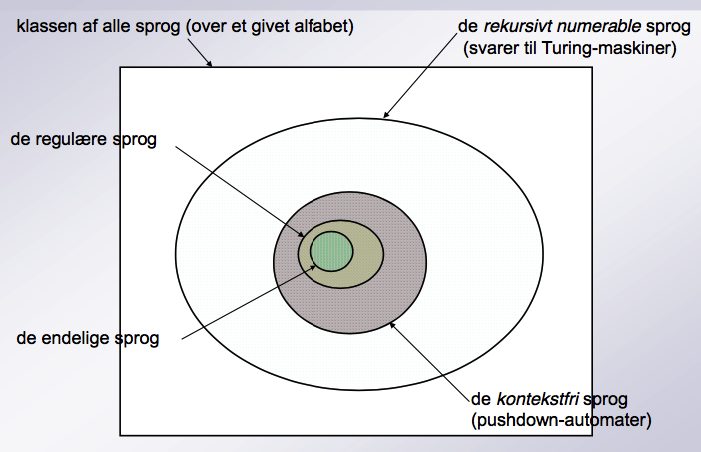
\includegraphics[width=70mm]{img/sprogklasser.png}
	  \caption{Klasser af formelle sprog	\label{formelleSprog1}}
  \end{figure}
  \end{itemize}
  \subsection{Endelige automater}
  \begin{itemize}
    \item En endelig automat accepterer et regulært sprog, hvorimod et regulært udtryk beskriver det og
    \item En endelig automat og et regulært udtryk har samme udtrykskraft, det vil sige, at de kan beskrive den samme mængde sprog. 
    \item Givet en streng svarer den enten ja eller nej
    \item Eksempel på en endelig automat over alphabet $\Sigma=\{0,1\}$, der accepterer en streng med et lige antal 0'er
    \begin{figure}[ht!]
	  \centering
	  \includegraphics[width=60mm]{img/FAeks.png}
	  \caption{Eksempel på en endelig automat	\label{FAeks2}}
    \end{figure}
    \item En finite automat er en 5-tuple $(Q, \Sigma, q_0, A, \delta)$
    \begin{itemize}
	    \item $Q$ er et endeligt mængde tilstande
      \item $\Sigma$ er et alfabet
      \item $q_0 \in Q$ er start-tilstanden
      \item $A \subseteq Q$ er endelig mængden af accept tilstande
      \item $\delta: Q \times \Sigma \rightarrow Q$ er transitionsfunktionen, som givet en tilstand og et tegn returnerer en tilstand. 
    \end{itemize}
    \item Den udvidet transitionsfunktion: $\delta^*: Q \times \Sigma^* \rightarrow Q$ er defineret på følgende måde for alle $q\in Q$ og $x \in \Sigma^*$
 	 	\begin{equation*}
		\delta(q,x) =
		\begin{cases}
			\mbox{$q$} & \mbox{hvis $x = \Lambda$} \\
			\mbox{$\delta(\delta^*(q,y),\sigma)$} & \mbox{hvis $x=y\sigma$ for alle $\sigma \in \Sigma$ og $y\in \Sigma^*$} \\
		\end{cases}
		\end{equation*}
    \item Sproget for en endelig automat M er defineret på følgende måde:
    \begin{equation*}
      L(M)=\{x \in \Sigma^* \ | \ \delta^*(q_0,x)\in A \}
    \end{equation*}

\subsection{Forskellige slags automater}
    \item En NFA er en FA, hvor outputtet af transitionsfunktionen er en mængde af tilstande
    \begin{itemize}
  	  \item Den kan have $\Lambda$-transitioner, som er transitioner, som gør det muligt at skifte tilstand på den tommestreng
      \item Man kan ved hjælp af $\Lambda$-eliminering, som er ren algoritme, der fjerner $\Lambda$-transitioner fra en NFA, få en NFA$^*$, som er en NFA uden   $\Lambda$-transitioner 
      \item Man kan ud fra NFA$^*$ få en FA, ved brug af determinisering (delmængdekonstruktionen)
      \item Derved har NFAer, NFA$^*$er og FAer samme udtrykningskraft og derved kan de bruges til at bevis kleenessætning, som lyder:
      \begin{itemize}
    	  \item For et hvert alfabeter $\Sigma$, kan alle regulære udtryk over $\Sigma$ blive accepteret af en endelig automat
      \end{itemize}
     \end{itemize}
  \end{itemize}
  \begin{figure}[ht!]
	  \centering
	  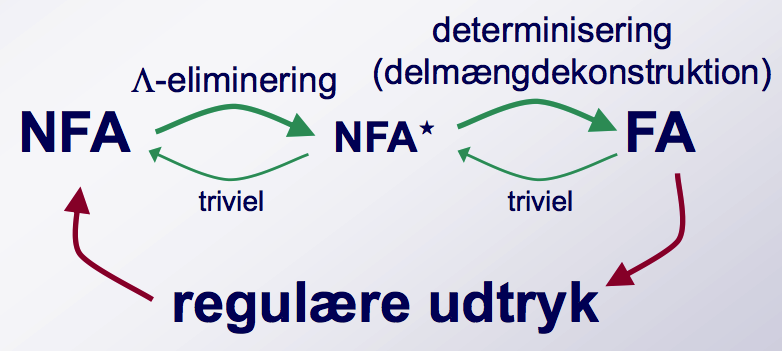
\includegraphics[width=100mm]{img/automater}
	  \caption{Forholdet mellem forskellige automater	\label{automater2}}
  \end{figure}
 
\subsection{Determinisering}
\begin{itemize}
  \item For at lave en NFA$^*$ om til en FA bruger man følgende algoritme
  \item Givet en NFA$^*$ $M=(Q,\Sigma,q_0,A,\delta)$ definer en FA $M_1=(Q_1,\sigma, q_1,A_1,\delta_1)$ ved 
  \begin{align*}
    Q &= 2^Q \\
    q_1 &= \{q_0\} \\
    A_1 &= \{ q\in Q \ | \ q \cup Q \neq \emptyset \} \\
    \delta_1(q,a)&=\bigcup_{r\in q}\delta(r,a)
  \end{align*}
  \item Hver tilstand i FA'en er en mængde af tilstande fra NFA'en
  \item Det gælder nu at $L(M)=L(M_1)$
\end{itemize}

\subsubsection{Bevis}
  Pr defination af L() for NFA'er og Fa'er: 
  \begin{align*}
    L(M)&=\{  x\in \Sigma^* \ | \ \delta^*(q_0,x) \cap A \neq \emptyset \} \\
    L(M_1)&=\{ x\in \Sigma ^* \ | \ \delta_1^*(q_1,x)\in A_1 \} 
  \end{align*}
  For at bevise determiniseringen skal bruge dette lemma:
  \begin{equation*}
  \forall x \in \Sigma^*: \delta_1^*(q_1,x) =  \delta^*(q_0,x)
  \end{equation*}
  som her er bevist ved hjælp af et induktionsbevis i strukturen af x: \\
  \textbf{Basis:} \\
  $x=\Lambda$:
  \begin{align*}
    \delta^*_1(q_1,\Lambda) &=  \delta^*(q_0,\Lambda) \\
    q_1 &= \text{(Def af $q_1$)} \\
    \{q_0\} &= \text{(Def af $\delta^*$ på $\Lambda$)} \\
    \delta^*(q_0,\Lambda) &= \\
  \end{align*}
  \textbf{IS.}: \\
  \textbf{IH.}: $\delta_1^*(q_1,y) =  \delta^*(q_0,y)$ \\
  $x=y\sigma$:
  \begin{align*}
    \delta_1^*(q_1,y\sigma)&=\delta^*(q_0,y\sigma) \\
    \delta_1(\delta_1^*(q_1,y),\sigma) &= \text{(IH.)} \\
    \delta_1(\delta^*(q_0,y),\sigma) &= \text{(Def. af $\delta_1$)}\\
    \bigcup_{r\in \delta^*(q_0,y)}\delta(r,a) &= \text{(Def. af $\delta$)}\\
    \delta^*(q_0,y\sigma) &= \\
  \end{align*}
  Vi kan nu bruge lemma'et til at bevise at $L(M)=L(M_1)$:
  \begin{align*}
    \delta_1(q_1,x)\in A_1 &\Updownarrow \text{(Lemma)} \\  
    \delta(q_0,x)\in A_1 &\Updownarrow \text{(Def. af $A_1$)} \\
    \delta(q_0,x)\cap A \neq \emptyset \\
  \end{align*}
   
\newpage
\subsection{Disposition}
\begin{enumerate}
  \item Regulære sprog
  \item Endelig automater 
  \item Forskellige slags automater 
  \item Determinisering 
  \item Determinisering bevis
\end{enumerate}

\newpage
\section{Lukkedhedsegenskaber}

\subsection{Regulære sprog}
  \begin{itemize}
    \item Et sprog S er et regulært sprog, hvis det kan beskrives af et regulært udtryk
    \item Sproget L(r) over et regulært udtryk er defineret i strukturen af r, således: 
    \begin{itemize}
      \item $L(\emptyset)=\emptyset $
      \item $L(\Lambda)=\{ \Lambda \}$
      \item $L(a)=\{a\}$
      \item $L(r_1+r_2)=L(r_1)\cup L(r_2)$
      \item $L(r_1r_2)=L(r_1)L(r_2)$
      \item $L(r_1^*)=L(r_1)^*$
    \end{itemize}
    \item $L(\emptyset^*)=L(\Lambda)$ så $\Lambda$ kan betragtes, som en forkortelse af $\emptyset^*$
    \item Operationer på regulære sprog
    \begin{itemize}
	    \item Foreningsoperation: givet to sprog $L_1,L_2\subseteq \Sigma^*$, så er forening af de to sprog defineret ved:
      \begin{equation*}
        L_1\cup L_2 = \{x \ | \ x\in L_1 \lor x\in L_2 \}
      \end{equation*}
      \item Konkateneringsoperation: givet to sprog $L_1,L_2\subseteq \Sigma^*$, så er konkateneringen af de to sprog defineret ved:
      \begin{equation*}
        L_1L_2= \{xy \ | \ x\in L_1 \land y\in L_2 \}
       \end{equation*}
      \item Kleenesstjerneoperation: givet et sprog $L \subseteq \Sigma^*$, så er Kleene stjerne af det sprog defineret ved:
      \begin{align*}
        L^* &= \bigcup_{i=0}^{\infty} L^i \\
            &= L^0\cup L^1 \cup L^2 \cup L^3  \\
            &= \{\Lambda \} \cup L \cup LL \cup LLL 
      \end{align*}
    \end{itemize}
    \item Klasser af formelle sprog:
    \begin{figure}[ht!]
	  \centering
	  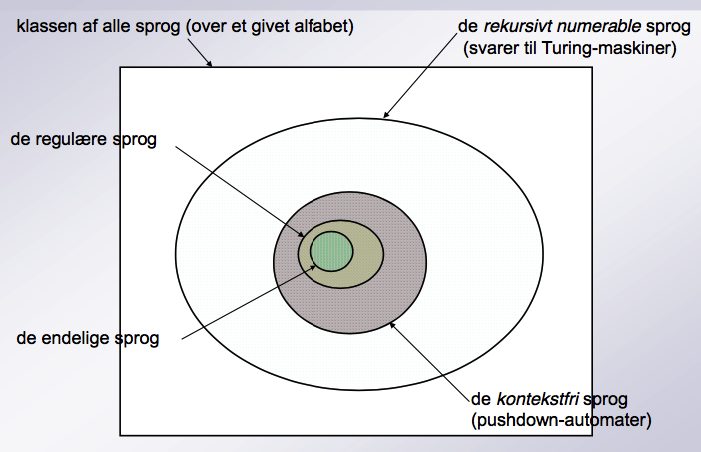
\includegraphics[width=70mm]{img/sprogklasser.png}
	  \caption{Klasser af formelle sprog	\label{formelleSprog}}
  \end{figure}
  \end{itemize}

\subsection{Lukkedhedsegenskaber for regulære sprog}
\begin{itemize}
  \item Når er sprog er lukkede under en operation, betyder det at outputtet givet en eller flere af den pågældende sprog også kan beskrives af det pågældende sprog.
  \item De regulære sprog er lukkede under de følgende operationer
  \begin{itemize}
    \item Forening
    \item Fællesmængde
    \item Minus
    \item Komplement
    \item Konkatanering
    \item kleene stjerne
  \end{itemize}
  \item Når man har bevist, at det regulære sprog er lukkede under en bestemt operation kan de bruges til at bevise at noget ikke er regulært
  \item Eksempel
  \begin{itemize}
    \item Hvis $L_1$ er regulært, $L_3$ ikke er regulært og $L_1 \cup L_2 = L_3$ medfører det, at $L_3$ ikke er regulært 
  \end{itemize}
  \item De regulære sprog er desuden lukket under homomorfi
  \item En homomorfi er defineret på følgende måde
  \begin{itemize}
    \item Antag at $g: \Sigma_1 \rightarrow \Sigma_2$
    \item Vi definer h på følgende måde
 	 	\begin{equation*}
		h(x) =
		\begin{cases}
			\mbox{$\Lambda$} & \mbox{hvis $x = \Lambda$} \\
			\mbox{$h(y)g(a)$} & \mbox{hvis $x=ya$, $y \in \Sigma_1^*$, $a \in \Sigma_1$} \\
		\end{cases}
		\end{equation*}    
  \end{itemize}
\end{itemize}

\subsection{Lukkedhedsegenskaber for kontekstfrie grammatikker}
\begin{itemize}
  \item De kontekstfrie grammatikker er lukkede under 
  \begin{itemize}
    \item forening
    \item Konkatanering
    \item kleene stjerne
  \end{itemize}
  \item Modsat regulære sprog er kontekstfrie grammatikker ikke lukkede under:  
  \begin{itemize}
    \item Fællesmængde
    \item Komplement
  \end{itemize}
  \item Kontekstfrie grammatikker kan bevises ved dette modeksempel
    \begin{enumerate}
    	\item $L_1= \{a^ib^jc^k \ | \ i<j \}$: som er en kontekstfri grammatik
    	\item $L_2= \{a^ib^jc^k \ | \ j<k \}$: som er en kontekstfri grammatik
      \item $L_1 \cap L_2 = \{a^ib^jc^k \ | \ i<j<k \}$, som ikke er en kontekstfri grammatik (kan bevises ved hjælp af pumping lemmaet)
    \end{enumerate}
  \item Det at kontekstfrie grammatikker ikke er lukkede under Komplement kan bevises på følgende måde med et lille modstridsbevis
  \begin{equation*}
    (L_1' \cup L_2')' = L_1 \cap L_2
  \end{equation*}
\end{itemize}

\subsection{Produktkonstruktionen}
\begin{itemize}
  \item Produktkonstruktionen gør det muligt at lave en union, intersection eller minus mellem to endelige automater $M_1=(Q_1,\Sigma,q_1,A_1,\delta_1)$ og $M_2=(Q_2,\Sigma,q_2,A_2,\delta_2)$
  \item Den resulterende endelig automat $M=(Q,\Sigma,q_0,A,\delta)$ bliver defineret på følgende måde
  \begin{align*}
    Q &= Q_1\times Q_2 \\
    q_0 &= (q_1,q_2) \\
  \end{align*}
  \item Transitionsfunktionen $\delta$ er defineret på følgende måde
  \begin{equation*}
    \delta((p,q),\sigma)=(\delta(p,\sigma),\delta(q,\sigma))
  \end{equation*}
  \item for alle $p \in Q_1$, $p \in Q_2$ og $\sigma \in \Sigma$
  \item Accept tilsandende er defineret på følgende måder for de forskellige operationer:
  \begin{enumerate}
    \item Hvis $A=\{(p,q) \ | \ p \in A_1 \lor p \in A_2  \}$ accepterer $M$ sproget $L(M_1) \cup L(M_2)$
    \item Hvis $A=\{(p,q) \ | \ p \in A_1 \land p \in A_2  \}$ accepterer $M$ sproget $L(M_1) \cap L(M_2)$
    \item Hvis $A=\{(p,q) \ | \ p \in A_1 \land p \notin A_2  \}$ accepterer $M$ sproget $L(M_1) - L(M_2)$    
  \end{enumerate}
\end{itemize}

\subsubsection{Bevis}
For at bevise produktkonstruktionen, skal vi vise, at hvis vi kører en streng igennem automaten svarer det til at køre en streng igennem begge automater. Vi skal derfor bevise denne sætning:

\begin{equation*}
  \delta^*((p,q),x)=  (\delta^*_1(p,x),  \delta_2^*(q,x))
\end{equation*}
\\
\textbf{Basis:}\\
$x=\Lambda$: 
\begin{align*}
  \delta^*((p,q),\Lambda) &= (\delta^*_1(p,\Lambda),  \delta_2^*(q,\Lambda))\\
  (p,q) &= (p,q)
\end{align*}
\textbf{I.S}: \\
\textbf{I.H}: $\delta^*((p,q),y) = (\delta^*_1(p,y),  \delta_2^*(q,y))$ \\
$x=y\sigma$:
\begin{align*}
  \delta^*((p,q),y\sigma) &=  (\delta^*_1(p,y\sigma),  \delta_2^*(q,y\sigma)) \\
  \delta(\delta^*((p,q),y), \sigma) &= \text{(IH.)} \\
  \delta((\delta^*_1(p,y),  \delta_2^*(q,y))), \sigma) &= \text{(Definationen af $\delta$ for prod)} \\
  (\delta_1(\delta^*_1(p,y), \sigma), \delta_2(\delta^*_2(q,y), \sigma)) &= \text{(Definationen af $\delta$ gennerelt)} \\
  (\delta^*_1(p,y\sigma),  \delta_2^*(q,y\sigma)) &=  
\end{align*}

\newpage
\subsection{Disposition}
\begin{enumerate}
  \item Regulære sprog
  \item Lukkedhedsegenskaber for regulære sprog
  \item Produktkonstruktionen
  \item Bevis for produktkonstruktionen 
  \item Evt. lukkedhedsegenskaber for CFGer
\end{enumerate}

\newpage
\section{Nondeterministiske automater}

\subsection{Nondeterministiske automater gennerelt}
\begin{itemize}
  \item Nondeterministiske automater kan beskrive samme mængde sprog, som regulære udtryk og endelig automater
  \begin{figure}[h]
	  \centering
	  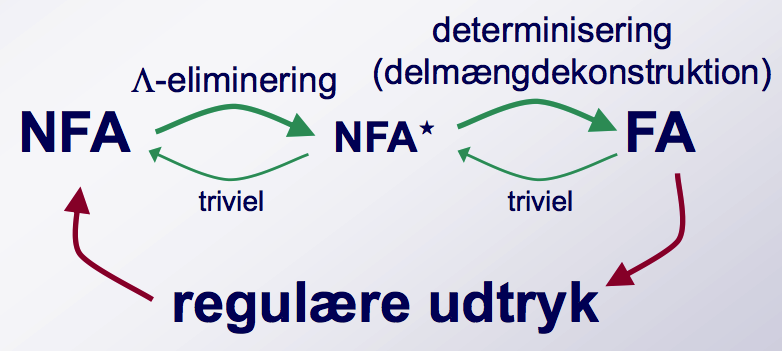
\includegraphics[width=100mm]{img/automater}
	  \caption{Forhold mellem forskellige automater	\label{automaterNFA}}
  \end{figure}
  \item En nondeterministisk automat er defineret, som en 5 tuple $(Q,\Sigma,q_0,A,\delta)$, hvor
  \begin{itemize}
    \item $Q$ er et finite sæt tilstande
    \item $\Sigma$ er en alphabet
    \item $q_0\in Q$ er starttilstanden
    \item $A \subseteq Q$ er et sæt accept tilstande
    \item $\delta: Q \times(\{ \Lambda \} \cup \Sigma) \rightarrow 2^Q$ er transitionsfunktionene
  \end{itemize}
  \item Den største forskel mellem en nondeterministisk automat og en endelig automat er transitionsfunktionen
  \begin{itemize}
    \item Transitionsfunktionens output er ikke længere en tilstand men et sæt af tilstande 
    \item For en tilstand kan der være ingen eller flere udgange på et symbol
    \item Der eksisterer $\Lambda$-transitioner, som gør at man kan skifte tilstand uden at få et input
  \end{itemize}
  \item $\Lambda$-lukning på et set af states er de tilstande, man kan komme til uden at bruge et tegn.
  \item Hvis $M=(Q, \Sigma, q_0, A, \delta)$ er en NFA, $S\subseteq Q$ er et sæt af tilstande, så er $\Lambda$-lukning på sættet $\Lambda(S)$ defineret på følgende måde
  \begin{enumerate}
    \item $S \subseteq \Lambda(S)$
    \item For alle $q \in \Lambda(S)$, $\delta(q,\Lambda) \subseteq \Lambda(S)$
  \end{enumerate}
  \item Den udvidet transitionsfunktionen  $\delta^*$ for en NFA $M=(Q, \Sigma, q_0, A, \delta)$ er defineret på følgende måde:
  \begin{equation*}
  	\delta^*(q,x) =
  		\begin{cases}
  			\mbox{$\Lambda(\{q\})$} & \mbox{hvis $x = \Lambda$} \\
  			\mbox{$\Lambda(\bigcup_{r \in \delta^*(q,y)}\delta(r,\sigma))$} & \mbox{hvis $x = y\sigma$ hvor $\sigma \in \Sigma$ og $y \in \Sigma^*$} \\
  		\end{cases}
  \end{equation*}    
  
  \item Sproget for en nondeterministisk automat $M$ er defineret på følgende måde
  \begin{equation*}
    L(M)=\{ x \in \Sigma^*  \ | \ \delta^*(q,x) \cap A \ne \emptyset \}
  \end{equation*}
\end{itemize}


\subsection{Determinisering}
\begin{itemize}
  \item For at lave en NFA$^*$ om til en FA bruger man følgende algoritme
  \item Givet en NFA$^*$ $M=(Q,\Sigma,q_0,A,\delta)$ definer en FA $M_1=(Q_1,\Sigma, q_1,A_1,\delta_1)$ ved 
  \begin{align*}
    Q &= 2^Q \\
    q_1 &= \{q_0\} \\
    A_1 &= \{ q\in Q \ | \ q \cup Q \neq \emptyset \} \\
    \delta_1(q,a)&=\bigcup_{r\in q}\delta(r,a)
  \end{align*}
  \item Hver tilstand i FA'en er en mængde af tilstande fra NFA'en
  \item Det gælder nu at $L(M)=L(M_1)$
\end{itemize}

\subsubsection{Bevis}
  Pr defination af L() for NFA'er og Fa'er: 
  \begin{align*}
    L(M)&=\{  x\in \Sigma^* \ | \ \delta^*(q_0,x) \cap A \neq \emptyset \} \\
    L(M_1)&=\{x\in \Sigma ^* \ | \ \delta_1^*(q_1,x)\in A_1 \} 
  \end{align*}
  For at bevise determiniseringen skal bruge dette lemma:
  \begin{equation*}
  \forall x \in \Sigma^*: \delta_1^*(q_1,x) =  \delta^*(q_0,x)
  \end{equation*}
  som her er bevist ved hjælp af et induktionsbevis i strukturen af x: \\
  \textbf{Basis:} \\
  $x=\Lambda$:
  \begin{align*}
    \delta^*_1(q_1,\Lambda) &=  \delta^*(q_0,\Lambda) \\
    q_1 &= \text{(Def af $q_1$)} \\
    \{q_0\} &= \text{(Def af $\delta^*$ på $\Lambda$)} \\
    \delta^*(q_0,\Lambda) &= \\
  \end{align*}
  \textbf{IS.}: \\
  \textbf{IH.}: $\delta_1^*(q_1,y) =  \delta^*(q_0,y)$ \\
  $x=y\sigma$:
  \begin{align*}
    \delta_1^*(q_1,y\sigma)&=\delta^*(q_0,y\sigma) \\
    \delta_1(\delta_1^*(q_1,y),\sigma) &= \text{(IH.)} \\
    \delta_1(\delta^*(q_0,y),\sigma) &= \text{(Def. af $\delta_1$)}\\
    \bigcup_{r\in \delta^*(q_0,y)}\delta(r,a) &= \text{(Def. af $\delta$)}\\
    \delta^*(q_0,y\sigma) &= \\
  \end{align*}
  Vi kan nu bruge lemma'et til at bevise at $L(M)=L(M_1)$:
  \begin{align*}
    x \in L(M_1) &\Updownarrow \\
    \delta_1(q_1,x)\in A_1 &\Updownarrow \text{(Lemma)} \\  
    \delta(q_0,x)\in A_1 &\Updownarrow \text{(Def. af $A_1$)} \\
    \delta(q_0,x)\cap A \neq \emptyset &\Updownarrow \\
    x \in L(M) &
  \end{align*}

\subsection{$\Lambda$-eliminering}
\begin{itemize}
  \item $\Lambda$ eliminering er en procedure, hvor man fjerner alle $\Lambda$-transitioner fra en NFA og man får derved en NFA$^*$, som er en NFA uden $\Lambda$-transitioner.
  \item For at lave $\Lambda$-eliminering på en automat, hvor man er givet en NFA $M=(Q_1,\Sigma,q_1,A_1,\delta_1)$ definerer en NFA$^*$ $N=(Q,\Sigma,q_0,A,\delta)$ således følgende gælder
  \begin{align*}
    Q &= Q_1 \\
    q_0 &= q_1 
  \end{align*}
  \item Desuden er transitionsfunktionen defineret således: $\delta(q,a) = \delta_1^*(q,a)$, for alle $q \in Q$ og alle $a\in \Sigma$
  \item Sættet af accept tilstande er defineret således afhængig om $\Lambda$ er indeholdt i sproget
  \begin{equation*}
  	A =
  		\begin{cases}
  			\mbox{$A_1 \cup {q_0}$} & \mbox{hvis $\Lambda(\{q_0\})\cap A_1 \ne \emptyset$} \\
  			\mbox{$A_1$} & \mbox{ellers} \\
  		\end{cases}
  \end{equation*}    
  \item Eksempel
  \begin{center}  
    \begin{tikzpicture}[>=stealth',shorten >=1pt,auto,node distance=2cm]
    \node[initial,state] (q0)      {$q_0$};
    \node[state]         (q1) [right of=q0]  {$q_1$};
    \node[state]         (q2) [right of=q1] {$q_2$};
    \node[accepting, state]         (q3) [right of=q2] {$q_3$};
    \path[->] 
          (q0) edge              node {a} (q1)
               edge [bend left]  node {$\Lambda$} (q3)
          (q1) edge              node {$\Lambda$} (q2)
          (q2) edge              node {b} (q3);
    \end{tikzpicture}
    \begin{tikzpicture}[>=stealth',shorten >=1pt,auto,node distance=2cm]
    \node[initial, accepting, state] (q0)      {$q_0$};
    \node[state]         (q1) [right of=q0]  {$q_1$};
    \node[state]         (q2) [right of=q1] {$q_2$};
    \node[accepting, state]         (q3) [right of=q2] {$q_3$};
    \path[->] 
          (q0) edge              node {a} (q1)
               edge [bend left]  node {a} (q2)
          (q1) edge [bend right]  node {b} (q3)
          (q2) edge              node {b} (q3);
    \end{tikzpicture}
  \end{center}
\end{itemize}
\subsubsection{Bevis}
  Bevis for $\delta^*(q,x)=\delta_1^*(q,x)$ for $|x| \geq 1$, da det ikke vil være tilfældet $\Lambda$ \\
  \textbf{Basis:} \\
  $x=\sigma$ hvor $\sigma \in \Sigma$:
  \begin{align*}
    \delta^*(q,\sigma) &= \delta^*(q,\sigma) \\
    \delta_1(q,\sigma) &=
    \delta_1^*(q,\sigma) &=
  \end{align*}
  \textbf{Induktionskridtet}:
  \textbf{IH.}: $\delta_1^*(q,y)=\delta_1^*(q,y)$ \\
  $x=y\sigma$:
  \begin{align*}
    \delta_1^*(q,y\sigma)&=\delta_1^*(q,y\sigma) \\
    \delta_1(\delta_1^*(q,y),\sigma))&= \text{(IH.)}  \\
    \delta_1(\delta^*(q,y),\sigma)&= \text{(Def af $\delta_1$)} \\
    \delta^*(\delta^*(q,y),\sigma)&= \text{(Def af $\delta^*$ for NFAer)}\\
    \Lambda(\bigcup_{r \in \delta^*(\delta^*(q,y), \Lambda)}\delta(r,\sigma))  &= \text{(Def af $\delta^*$ på $\Lambda$)} \\
    \Lambda(\bigcup_{r \in \Lambda(\delta^*(q,y))}\delta(r,\sigma)) &= \text{(Def af $\delta^*$)} \\ 
    \Lambda(\bigcup_{r \in \delta^*(q,y)}\delta(r,\sigma)) &= \text{(Def. af $\delta^*$)} \\
    \delta_1^*(q,y\sigma) &= \\
  \end{align*}  

\newpage
\subsection{Disposition}
\begin{enumerate}
  \item NFAer gennerelt
  \item Lambda eliminering 
  \item Determinisering
  \item Determiniseringsbevis
  \item Evt. Kleenes sætning og bevis
\end{enumerate}

\newpage
\section{Minimering af automater}

\subsection{Endelige automater}
  \begin{itemize}
    \item En endelig automat accepterer et regulært sprog, hvorimod et regulært udtryk beskriver det og
    \item En endelig automat og et regulært udtryk har samme udtrykskraft, det vil sige, at de kan beskrive den samme mængde sprog. 
    \item Givet en streng svarer den enten ja eller nej
    \item Eksempel på en endelig automat over alphabet $\Sigma=\{0,1\}$, der accepterer en streng med et lige antal 0'er
    \begin{figure}[ht!]
	  \centering
	  \includegraphics[width=60mm]{img/FAeks.png}
	  \caption{Eksempel på en endelig automat	\label{FAeks2}}
    \end{figure}
    \item En finite automat er en 5-tuple $(Q, \Sigma, q_0, A, \delta)$
    \begin{itemize}
	    \item $Q$ er et endeligt mængde tilstande
      \item $\Sigma$ er et alfabet
      \item $q_0 \in Q$ er start-tilstanden
      \item $A \subseteq Q$ er endelig mængden af accept tilstande
      \item $\delta: Q \times \Sigma \rightarrow Q$ er transitionsfunktionen, som givet en tilstand og et tegn returnerer en tilstand. 
    \end{itemize}
    \item Den udvidet transitionsfunktion: $\delta^*: Q \times \Sigma^* \rightarrow Q$ er defineret på følgende måde for alle $q\in Q$ og $x \in \Sigma^*$
 	 	\begin{equation*}
		\delta(q,x) =
		\begin{cases}
			\mbox{$q$} & \mbox{hvis $x = \Lambda$} \\
			\mbox{$\delta(\delta^*(q,y),\sigma)$} & \mbox{hvis $x=y\sigma$ for alle $\sigma \in \Sigma$ og $y\in \Sigma^*$} \\
		\end{cases}
		\end{equation*}
    \item Sproget for en endelig automat M er defineret på følgende måde:
    \begin{equation*}
      L(M)=\{x \in \Sigma^* \ | \ \delta^*(q_0,x)\in A \}
    \end{equation*}
  \end{itemize}

\subsection{L-skelnelighed}
  \begin{itemize}
    \item Hvis to strenge x og y, er L-skelnelig betyder det, at der findes et streng $z \in \Sigma^*$, så en af de følgende til gælder
     \begin{enumerate}
       \item $xz \in L$ og $yz \notin L$
       \item $xz \notin L$ og $yz \in L$
     \end{enumerate}
    \item Hvis man har et en endelig automat $M=(Q,\Sigma,q_0,A,\delta)$, som accepterer sproget $L\subseteq\Sigma^*$ og hvis strengene x og y er L-skelnelig, så gælder der at $\delta^*(q_0,x) \neq \delta^*(q_0,y) $. 
    \begin{itemize}
      \item For $n \geq 2$, hvis der er et sæt af L-skelnelig strenge, skal der mindst være n tilstande i den endelige automaten, der acceptere sproget.
    \end{itemize}
    \item Hvis man har et uendeligt sæt af parvis L-skelnelig strenge betyder det, at sproget ikke kan blive accepteret af en endelig automat 
  \end{itemize}


\subsection{Ækvivalensklasser og relationer}
\begin{itemize}
  \item En relation R mellem to elementer a og b er skrevet på følgende måde $aRb$
  \item En ækvivalensrelation R på et sæt S er en relation, som har følgende egenskaber:
  \begin{enumerate}
    \item R er refleksiv: for alle $x \in S$, $xRx$
    \item R er symmetrisk: for alle $x,y \in S$ hvis $xRy$, så gælder $yRx$
    \item R er transitiv: for alle $x,y,z \in S$ hvis $xRy$ og $yRz$ så gælder $xRz$
  \end{enumerate}
  \item En ækvivalensklasse $R$ over et sæt $S$, som indeholder x er beskrevet på følgende måde
  \begin{equation*}
    [x]_R=\{ y \in S \ | \ yRx  \}
  \end{equation*}
  \item For et sprog L har vi defineret ækvivalensrelationen $I_l$ på $\Sigma^*$, på følgende måde:
  \begin{itemize}
    \item $xI_Ly$ hvis og kun hvis $x$ og $y$ er L-uskelnelig
  \end{itemize}
  \item Hvis to strenge x og y er L-uskelnelig betyder det at følgende gælder
  \begin{equation*}
    \forall z \in \Sigma^*: x \in L \Leftrightarrow  y \in L
  \end{equation*}
  \item \textbf{Myhill-Nerode Theoremet} siger, at hvis og kun hvis sættet af ækvivalensklasser $Q_L$ over relationen $I_L$ på $\Sigma^*$ er endeligt kan sproget blive accepteret af en FA. 
  \begin{itemize}
    \item Hvis sættet $Q_L$ er endeligt, så kan man lave en endelig automat vha Myhill-Nerode konstruktioen $M_L=(Q_L,\Sigma,q_0,A,\delta)$, som accepter L hvor følgende gælder 
    \begin{align*}
      q_0 &= [\Lambda] \\
      A &= \{ q \in Q_L \ | \ q \subseteq L \}
    \end{align*}
    \item Transitionsfunktionen er defineret på følgende måde for alle $a \in \Sigma$ og $x \in \Sigma^*$
    \begin{equation*}
      \delta([x], a) = [xa]
    \end{equation*}
    \item Desuden har FAen det mindst mulige antal tilstande 
  \end{itemize}
\end{itemize}

\subsection{Minimeringsalgoritmen}
\begin{itemize}
  \item Man bruger den følgende notation til at beskrive de strenge, der får en FA til at være i en tilstand q
  \begin{equation*}
    L_q=\{x \in \Sigma^* \ | \ \delta(q_0,x)=q \}
  \end{equation*}
  \item Ækvivalensrelationen på $\Sigma^*$ giver os ækvivalensrelationen $\equiv$ på sættet Q af tilstande i M. For $p,q \in Q$
  \begin{itemize}
    \item $p \equiv q$, hvis og kun hvis strengen i $L_p$ og $L_q$ er i samme ækvivalensklasse. 
  \end{itemize}
  \item To tilstande $p,q \in Q$ er ikke ækvivalente, hvis strengene i $L_p$ og $L_q$ er L-skelnelig altså
  \begin{itemize}
    \item $p \not\equiv q$ hvis og kun hvis for en streng $z \in \Sigma^*$ præcis en af tilstandene $\delta(p,z)$ eller $\delta(q,z)$ er i A.
  \end{itemize}
  \item Minimeringsalgoritmen for en endelig automat indeholder følgende skridt
  \begin{enumerate}
    \item Fjern alle uopnåelige tilstande 
    \item Find $\equiv$ ved at udfylde en tabel over par af forskellige tilstande
    \item Kombinere tilstande, som svarer til de umærkede par   
  \end{enumerate}
  \item For at finde de tilstande, hvor $p \equiv q$ bruger man følgende algoritme, som består af følgende skridt
  \begin{enumerate}
    \item List alle par af par af forskellige tilstande 
    \item Første gang skal man marker alle de tilstande, hvor mindst en af tilstandene er i A, de er L-skelnelig i strengen $\Lambda$
    \item Man tjekker så for alle umærkede par $(s,r)$ om der er et symbol $\sigma \in \Sigma$, hvor $\delta(s,\sigma)=p$ og  $\delta(r,\sigma)=q$ hvor parret $(p,q)$ er blevet markerede 
    \begin{itemize}
      \item Dette gør man indtil der er en runde hvor der ikke bliver markerede flere par 
    \end{itemize}
   \end{enumerate}
\end{itemize}

\subsection{Bevis for Myhill-Nerode Konstruktionen}
Vi skal vise, at $x \in L(M_L) \Leftrightarrow x \in L$
\begin{align*}
  x \in L(M_L) &\Leftrightarrow \delta^*(q_0,x) \in A \\
  \text{(Def. af $q_0$)} &\Leftrightarrow \delta^*([\Lambda],x) \in A \\
  \text{(Def. af $\delta$)} &\Leftrightarrow [\Lambda x] \in A \\
  \text{(Def. af $\Lambda$)}  &\Leftrightarrow [x] \in A \\
  \text{(Def. af $A$)} &\Leftrightarrow [x] \cap L \neq \emptyset \\
  \text{(Bevis følger)} &\Leftrightarrow x \in L
\end{align*}
Dvs. $L=L(M_L)$ 
\\ \ \\
Bevis for $[x] \cap L \neq \emptyset \Leftrightarrow x \in L$
\begin{enumerate}
  \item $x \in L \Rightarrow x \cap L \neq \emptyset$ da $x \in [x]$
  \item $x \cap L \neq \emptyset \Rightarrow x \in L $, modstridsbevis:
  \begin{itemize}
    \item Antag $x \notin L$
    \item Lad $y \in [x] \cap L$, dvs. $y \in L$
    \item $\Lambda$ skelner x og y, så $y\notin [x]$ $\lightning$
  \end{itemize}
\end{enumerate}
Bevis for lemma ved strukturel induktion i y: 
\begin{equation*}
  \forall x,y \in \Sigma^*:\delta^*([x],y)=[xy]
\end{equation*}
\textbf{Basis:}
$y=\Lambda$ 
\begin{equation*}
  \delta^*([x],\Lambda) = [x] = [x\Lambda] 
\end{equation*}
\textbf{Induktionsskridt:}\\ 
\textbf{IH.}: $\Sigma^*:\delta^*([x],z)=[xz]$ \\
$y=z\sigma$:
\begin{align*}
  \delta^*([x],z\sigma) &= [xz\sigma] \\
  \delta(\delta^*([x],z),\sigma) &= \text{(IH.)} \\
  \delta([xz],\sigma) &= \text{(Def. af $\delta$)} \\
  [xz\sigma] &=
\end{align*}

\newpage
\subsection{Disposition}
\begin{enumerate}
  \item FAer
  \item Ækvivalensklasser
  \item Minimeringsalgoritmen 
  \item Myhill-Nerode Konstruktionen 
\end{enumerate}

\newpage  
\section{Begrænsninger af regulære sprog}
\subsection{Regulære sprog}
  \begin{itemize}
    \item Et sprog S er et regulært sprog, hvis det kan beskrives af et regulært udtryk
    \item Sproget L(r) over et regulært udtryk er defineret i strukturen af r, således: 
    \begin{itemize}
      \item $L(\emptyset)=\emptyset $
      \item $L(\Lambda)=\{ \Lambda \}$
      \item $L(a)=\{a\}$
      \item $L(r_1+r_2)=L(r_1)\cup L(r_2)$
      \item $L(r_1r_2)=L(r_1)L(r_2)$
      \item $L(r_1^*)=L(r_1)^*$
    \end{itemize}
    \item $L(\emptyset^*)=L(\Lambda)$ så $\Lambda$ kan betragtes, som en forkortelse af $\emptyset^*$
    \item Operationer på regulære sprog
    \begin{itemize}
	    \item Foreningsoperation: givet to sprog $L_1,L_2\subseteq \Sigma^*$, så er forening af de to sprog defineret ved:
      \begin{equation*}
        L_1\cup L_2 = \{x \ | \ x\in L_1 \lor x\in L_2 \}
      \end{equation*}
      \item Konkateneringsoperation: givet to sprog $L_1,L_2\subseteq \Sigma^*$, så er konkateneringen af de to sprog defineret ved:
      \begin{equation*}
        L_1L_2= \{xy \ | \ x\in L_1 \land y\in L_2 \}
       \end{equation*}
      \item Kleenesstjerneoperation: givet et sprog $L \subseteq \Sigma^*$, så er Kleene stjerne af det sprog defineret ved:
      \begin{align*}
        L^* &= \bigcup_{i=0}^{\infty} L^i \\
            &= L^0\cup L^1 \cup L^2 \cup L^3  \\
            &= \{\Lambda \} \cup L \cup LL \cup LLL 
      \end{align*}
    \end{itemize}
    \item Klasser af formelle sprog:
    \begin{figure}[ht!]
	  \centering
	  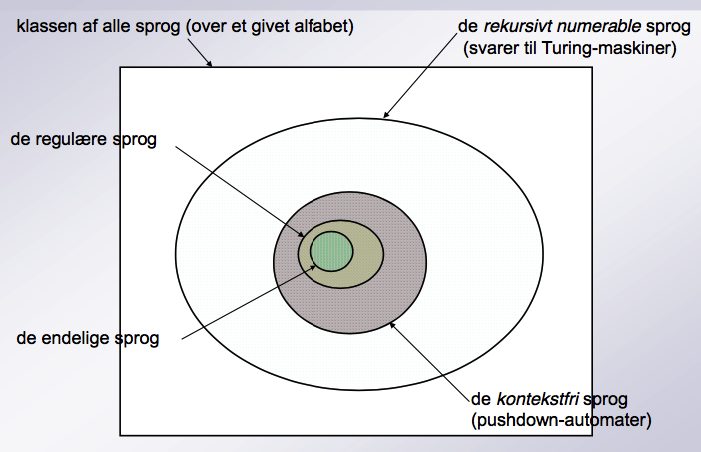
\includegraphics[width=70mm]{img/sprogklasser.png}
	  \caption{Klasser af formelle sprog	\label{formelleSprog}}
  \end{figure} 
  \end{itemize}

\subsection{Pumping lemmaet for regulære sprog}
\begin{itemize}
  \item Vi har en FA $M=(Q,\Sigma, q_0, A, \delta)$, som accepterer sproget $L \subseteq \Sigma^*$ og $|Q|=n$, så må der gælde
  \begin{enumerate}
  	\item Hvis strengen x, som bliver accepteret af M, hvor $|x|=n-1$, og har n forskellige prefixes, så må der tænkteligt, at FAen er i en ny tilstand efter hvert tegn
    \item Hvis $|x| \geq n$, så må den have gået igennem mindst en tilstand mindst 2 gang
    \begin{itemize}
	    \item Det må betyde, at der findes to forskellige prefix af strengen $u$ og $uv$, hvor følgende gælder $\delta(q_0,u)=\delta(q_0,uv)$, hvor $v \neq \Lambda$
      \item Altså er $x \in L$, når $x=uvw$ og derfor må der være et loop altså v, dermed må der gælde at strengen på form $uv^mw \in L$ 
      \item Desuden må det gælde, at $|uv| \leq n$
      \item Dette fortæller os, at der er mange flere strenge ud over $x$, der bliver accepteret af $m$
    \end{itemize}
  \end{enumerate}
  \item Dette bliver kaldt pumping lemmaet 
  \begin{figure}[h]
	  \centering
	  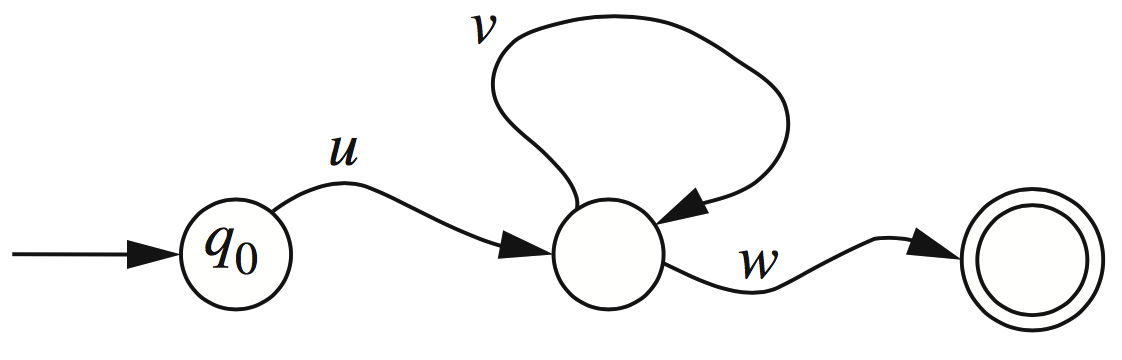
\includegraphics[width=100mm]{img/pumpingReg}
	  \caption{Pumping af en automat	\label{pumping1}}
  \end{figure}
  \item Dette lemma kan blive brugt i kontraponerede form til at bevise at noget ikke er regulært 
  \begin{itemize}
	  \item Da pumping lemma er opfyldt $\Rightarrow$ sproget er regulært gør at hvis sproget er ikke regulært $\Rightarrow$ pumping lemmaet er ikke opfyldt
  \end{itemize}
  \item Eksempel (bevis for $L=\{ x \in \Sigma^* \ | \ n_a(x) = n_b(x) \}$ ikke er regulært):
  \begin{itemize}
	  \item Vi skal vise, at det gælder for ethvert n
    \item Vi vælger strengen $x=a^nb^n$, dermed er $x\in L$ og $uv=a^{|uv|}$, da $|uv| \leq n$ og $|v| > 0$
    \item Vi vælger $m=2$ og strengen er ikke længere i sproget, da $a^{n+2|v|}b \notin L$, da  $n_a(x) \neq n_b(x)$
  \end{itemize}

\end{itemize}


\subsection{L-skelnelighed}
  \begin{itemize}
    \item Hvis to strenge x og y, er L-skelnelig betyder det, at der findes et streng $z \in \Sigma^*$, så en af de følgende til gælder
     \begin{enumerate}
       \item $xz \in L$ og $yz \notin L$
       \item $xz \notin L$ og $yz \in L$
     \end{enumerate}
    \item Hvis man har et en endelig automat $M=(Q,\Sigma,q_0,A,\delta)$, som accepterer sproget $L\subseteq\Sigma^*$ og hvis strengene x og y er L-skelnelig, så gælder der at $\delta^*(q_0,x) \neq \delta^*(q_0,y) $. 
    \begin{itemize}
      \item For $n \geq 2$, hvis der er et sæt af L-skelnelig strenge, skal der mindst være n tilstande i den endelige automaten, der acceptere sproget.
    \end{itemize}
    \item Hvis man har et uendeligt sæt af parvis L-skelnelig strenge betyder det, at sproget ikke kan blive accepteret af en endelig automat 
  \end{itemize}


\subsection{Ækvivalensklasser og relationer}
\begin{itemize}
  \item En relation R mellem to elementer a og b er skrevet på følgende måde $aRb$
  \item En ækvivalensrelation R på et sæt S er en relation, som har følgende egenskaber:
  \begin{enumerate}
    \item R er refleksiv: for alle $x \in S$, $xRx$
    \item R er symmetrisk: for alle $x,y \in S$ hvis $xRy$, så gælder $yRx$
    \item R er transitiv: for alle $x,y,z \in S$ hvis $xRy$ og $yRz$ så gælder $xRz$
  \end{enumerate}
  \item En ækvivalensklasse $R$ over et sæt $S$, som indeholder x er beskrevet på følgende måde
  \begin{equation*}
    [x]_R=\{ y \in S \ | \ yRx  \}
  \end{equation*}
  \item For et sprog L har vi defineret ækvivalensrelationen $I_l$ på $\Sigma^*$, på følgende måde:
  \begin{itemize}
    \item $xI_Ly$ hvis og kun hvis $x$ og $y$ er L-uskelnelig
  \end{itemize}
  \item Hvis to strenge x og y er L-uskelnelig betyder det at følgende gælder
  \begin{equation*}
    \forall z \in \Sigma^*: x \in L \Leftrightarrow  y \in L
  \end{equation*}
  \item \textbf{Myhill-Nerode Theoremet} siger, at hvis sættet at hvis og kun hvis sættet af ækvivalensklasser $Q_L$ over relationen $I_L$ på $\Sigma^*$ er endeligt kan sproget blive accepteret af en FA. 
  \begin{itemize}
    \item Hvis sættet $Q_L$ er endeligt, så kan man lave en endelig automat vha Myhill-Nerode konstruktioen $M_L=(Q_L,\Sigma,q_0,A,\delta)$, som accepter L hvor følgende gælder 
    \begin{align*}
      q_0 &= [\Lambda] \\
      A &= \{ q \in Q_L | q \subseteq L \}
    \end{align*}
    \item Transitionsfunktionen er defineret på følgende måde for alle $a \in \Sigma$ og $x \in \Sigma^*$
    \begin{equation*}
      \delta([x], a) = [xa]
    \end{equation*}
    \item Desuden har FAen det mindst mulige antal tilstande 
  \end{itemize}
\end{itemize}


\newpage
\subsection{Disposition}
\begin{enumerate}
  \item Regulære sprog
  \item Pumping lemmaet for regulære sprog
  \item L-skelnelighed
  \item Ækvivalensklasser og -relationer
\end{enumerate}

\newpage
\section{Kontektsfri grammatikker}
\subsection{Definition af kontektsfri grammatikker}
\begin{itemize}
	\item En kontekstfri grammatik er en 4 tuple $G=(V,\Sigma,S,P)$, hvor
  \begin{itemize}
  	\item $V$ og $\Sigma$ er endelig adskilte sæt
    \item $S \in V$
    \item $P$ er et endelig sæt af formularer på formen $A \rightarrow \alpha$, hvor $A \in V$ og $\alpha \in (V \cup \Sigma)^*$
  \end{itemize}
  \item Elementerne i $\Sigma$ bliver kaldt terminaler 
  \item Elementerne i $V$ bliver kaldt for nonterminaler eller variabler
  \item $S$ er start variablen 
  \item Elementerne i $P$ bliver kaldt grammaregler eller produktioner
  \item $\Rightarrow$ bliver brugt, som et skridt i en udledning af en streng
  \begin{itemize}
  	\item $\alpha \Rightarrow^n \beta $ referer til en sekvens af n skridt
    \item $\alpha \Rightarrow^* \beta $ referer til en sekvens af 0 eller flere skridt
    \item $\alpha \Rightarrow_G \beta$,  $\alpha \Rightarrow^n_G \beta$ eller  $\alpha \Rightarrow^*_G \beta$ bliver brugt til eksplicit at sige at grammaet $G$ bliver brugt 
  \end{itemize}
  \item Sproget af en kontekstfri grammatik $G=(V,\Sigma,S,P)$ er 
  \begin{equation*}
    L(G) = \{ x \in \Sigma \ | \ S \Rightarrow^*_G x\}
  \end{equation*}
  \item Et sprog er en kontekstfri sprog, hvis der findes en CFG, hvor L=L(G)
  \item De regulære sprog og finite sprog er indehold i de kontekstfrie sprog, dette kan bevises ved brug af de regulære grammatikker eller strukturel induktion i de regulære udtryk
    \begin{figure}[ht!]
	  \centering
	  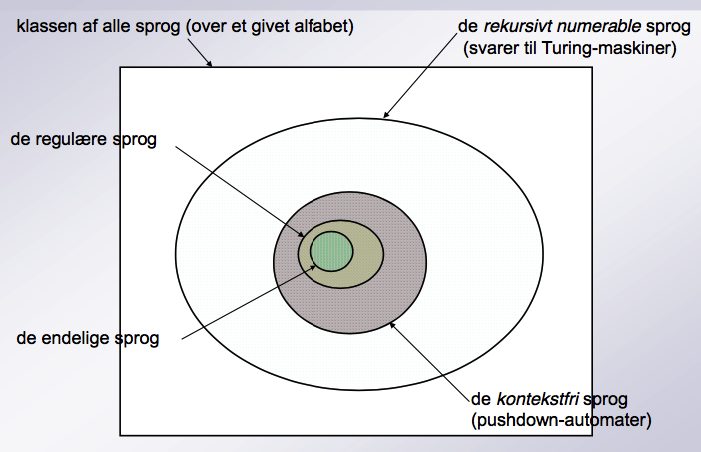
\includegraphics[width=70mm]{img/sprogklasser.png}
	  \caption{Klasser af formelle sprog	\label{formelleSprog}}
  \end{figure} 

\end{itemize}

\subsection{Derivationstræer og tvetydighed}
\begin{itemize}
	\item Derivationstræer er beskrivelsen af udledning af et ord for det kontekstfrie sprog ud fra grammaen 
  \item Hvis der findes mere en et derivationstræ for en streng i L(G), så er grammaen tretydig
  \item Eksempel:
  \begin{itemize}
  	\item Gramma: $S \rightarrow 1 \ | \ 0 \ | \ S + S \ | \ S-S $
    \item Sekvens: $S \Rightarrow^* 1+1-1$
    \item Træer: \\
    \begin{center}
      \Tree
      [.$S$ 
          [.$S$ [.$1$ ] ] 
          [.$+$ ] 
          [.$S$ [.$S$  [.$1$ ] ] 
                [.$-$ ] 
                [.$S$  [.$1$ ] ] ] 
        ] \qquad
      \Tree
      [.$S$ 
          [.$S$ [.$S$  [.$1$ ] ] 
                [.$+$ ] 
                [.$S$  [.$1$ ] ] ] 
          [.$-$ ] 
          [.$S$ [.$1$ ] ]
        ] \qquad
    \end{center}
  \end{itemize}
\end{itemize}

\subsection{Chompsky normal form}
\begin{itemize}
	\item En grammatik er på Chompsky normal form hvis hver produktion er på en af de to former
  \begin{itemize}
  	\item $A \rightarrow BC$ (Hvor B og C er nonterminaler)
    \item $A \rightarrow \sigma $ (Hvor $\sigma$ er en terminal)
  \end{itemize}
  \item For et hvert gramma $G$ findes, der en anden gramma $L(G_1)$ på chompsky normal form, hvor $L(G)=L(G_1)-\{\Lambda \}$
  \item For at lave et sprog, om til et sprog på Chompsky normal form omskriver man sproget i fire trin
  \begin{enumerate}
  	\item Ingen produktioner på form $A \rightarrow \Lambda$
    \begin{itemize}
    	\item For at fjerne disse produktioner, laver man ekstra produktioner, hvor den terminal, som kan blive til $\Lambda$ ikke er med.
      \item Derefter fjerner man alle $\Lambda$-transitionerne
    \end{itemize}
    \item Ingen produktioner på form $A \rightarrow B$
    \begin{itemize}
    	\item Alle de steder, hvor der er en unitproduktion, tilføjer man de produktioner, som den nonterminal der er resultatet af unitproduktionen har
      \item Derefter fjerne man alle unit produktioner
    \end{itemize}
    \item Alle produktioner på form $A \rightarrow B_1 ... B_n$ eller $A \rightarrow a$ hvor $n\geq 2$
    \begin{itemize}
    	\item Man laver nye terminaler, som har en produktion nemlig en nonterminal og erstatter nonterminalen med de produktioner de steder med nonterminaler, som ikke er på form $A \rightarrow a$
    \end{itemize}
    \item For alle produktioner på form $A \rightarrow B_1 ... B_n$, $n=2$
    \begin{itemize}
    	\item De steder med produktioner på følgende form $A \rightarrow B_1 ... B_n$, $n<2$ sætter man nonterminalerne ind i grupper par af to og erstatter de andre produktioner med disse 
    \end{itemize}
  \end{enumerate}
  \item Eksempel: 
   \begin{align*}
     S &\rightarrow ABA \\
     A &\rightarrow aAa  \ | \ \Lambda \\
     B &\rightarrow bBb  \ | \ \Lambda 
   \end{align*}
 \begin{enumerate}
   \item Fjern $\Lambda$-produktioner
   \begin{align*}
     S &\rightarrow ABA \ | \ AB  \ | \ BA \ | \ AA \ | \ A  \ | \ B \\
     A &\rightarrow aAa  \ | \ aa \\
     B &\rightarrow bBb  \ | \ bb 
   \end{align*}
   \item Fjern unit-produktioner
   \begin{align*}
     S &\rightarrow ABA \ | \ AB  \ | \ BA \ | \ AA \ | \  aAa  \ | \ aa  \ | \ bBb  \ | \ bb \\
     A &\rightarrow aAa  \ | \ aa \\
     B &\rightarrow bBb  \ | \ bb 
   \end{align*}
   \item Fjern produktioner på form $A \rightarrow a$
   \begin{align*}
     S &\rightarrow ABA \ | \ AB  \ | \ BA \ | \ AA \ | \  X_1AX_1  \ | \ X_1X_1  \ | \ X_2BX_2  \ | \ X_2X_2 \\
     A &\rightarrow X_1AX_1  \ | \ X_1X_1 \\
     B &\rightarrow X_2BX_2  \ | \ X_2X_2 \\
     X_1 &\rightarrow a \\
     X_2 &\rightarrow b 
   \end{align*}
   \item Alle produktioner på form $A \rightarrow B_1 ... B_n$, $n=2$
   \begin{align*}
     S &\rightarrow AZ_1 \ | \ AB  \ | \ BA \ | \ AA \ | \  X_1Z_2  \ | \ X_1X_1  \ | \ X_2Z_3  \ | \ X_2X_2 \\
     A &\rightarrow X_1Z_1  \ | \ X_1X_1 \\
     B &\rightarrow X_2Z_2  \ | \ X_2X_2 \\
     X_1 &\rightarrow a \\
     X_2 &\rightarrow b \\
     Z_1 &\rightarrow BA \\
     Z_2 &\rightarrow AX_1 \\
     Z_3 &\rightarrow BX_2 
   \end{align*}
   \end{enumerate}
  \item Hvis et gramma er på Chompsky Normal Form, så er alle derivationstræer et binærttræ
  \begin{itemize}
  	\item Alle blade svarer til et terminal symbol 
    \item Et binært træ med højde h har højest $2^h$-blade
  \end{itemize}
\end{itemize}

\subsection{Pumping lemmaet for kontektsfri grammatikker}
\begin{itemize}
  \item Vi antager for en kontekstfri grammatik G at
  \begin{itemize}
  	\item G er på Chompsky Normal Form
    \item G har i alt p nonterminalerne
    \item $\exists u \in L(G)$ hvor $|u| \geq 2^{p+1}$
  \end{itemize}
  \begin{figure}[ht]
    \centering
    \includegraphics[width=100mm]{img/Derivationstrae} 
  \end{figure}
  \item Så må der gælde for et derivationstræ T for U at 
  \begin{itemize}
  	\item Højden af T er mindst $p+1$
    \item Der findes en sti fra roden til u, hvor en nonterminal mindst indgår to gange
  \end{itemize}
  \item Vi kan ud fra disse observationer, inddele vores streng i 5 dele $u=vwxyz$ hvor
  \begin{itemize}
  	\item $|wy|>0$
    \item $wxy \leq 2^{p+1}$: på det nederste steder
    \item Det er muligt, at "Pumpe" w og y, så $u=vw^mxy^mz$ også er i sproget 
  \end{itemize}
  \item Vi har hermed fået udledt pumping lemmaet, hvor vi kalder $2^p$ for $n$, vi kan bruge dette lemma i kontraponerede form til at bevise at noget ikke er regulært
  \item Eksempel på brug til bevis:
  \begin{itemize}
  	\item $L = \{ a^ib^jc^k \ | \ i<j<l\}$
    \item $u = a^nb^{n+1}c^{n+2}$
    \item Alle mulige opdelinger valg af $vy$
    \begin{enumerate}
    	\item $vy=a^{|wy|}$: \\
      Vi vælger $m=2$, så $u = a^{n+|wy|}b^{n+1}c^{n+2}$ og da $|wy| > 0$ er $i\geq j$, har vi pumpet u ud af sproget
    	\item $vy=b^{|wy|}$: \\
      Vi vælger $m=0$, så  $u = a^{n}b^{n+1-|wy|}c^{n+2}$ og da $|wy| > 0$ er $j\leq i$, har vi pumpet u ud af sproget
    	\item $vy=c^{|wy|}$: \\
      Det samme som i b
    	\item $vy=a^kb^{k'}$: \\
      Vi vælger $m=2$, så $u= a^{n+k}b^{n+1+k'}c^{n+2}$, da $k>0 \land k'>0$ (ellers vil vi være i case 1 eller 2) er $j \geq l$, og u er pumpet ud af sproget
    	\item $vy=b^kc^{k'}$: \\
      Vi vælger $m=2$, så $u= a^{n}b^{n+1-k}c^{n+2-k'}$, da $k>0 \land k'>0$ (ellers vil vi være i case 2 eller 3) er $j \leq i$, og u er pumpet ud af sproget
    \end{enumerate}
  \end{itemize}
\end{itemize}
  
\subsection{Lukkedhedsegenskaber for kontekstfri grammatikker}
\begin{itemize}
  \item De kontekstfrie grammatikker er lukkede under 
  \begin{itemize}
    \item forening
    \item Konkatanering
    \item kleene stjerne
  \end{itemize}
  \item Modsat regulære sprog er kontekstfrie grammatikker ikke lukkede under:  
  \begin{itemize}
    \item Fællesmængde
    \item Komplement
  \end{itemize}
  \item Kontekstfrie grammatikker kan bevises ved dette modeksempel
    \begin{enumerate}
    	\item $L_1= \{a^ib^jc^k \ | \ i<j \}$: som er en kontekstfri grammatik
    	\item $L_2= \{a^ib^jc^k \ | \ j<k \}$: som er en kontekstfri grammatik
      \item $L_1 \cap L_2 = \{a^ib^jc^k \ | \ i<j<k \}$, som ikke er en kontekstfri grammatik (kan bevises ved hjælp af pumping lemmaet)
    \end{enumerate}
  \item Det at kontekstfrie grammatikker ikke er lukkede under Komplement kan bevises på følgende måde med et lille modstridsbevis
  \begin{equation*}
    (L_1' \cup L_2')' = L_1 \cap L_2
  \end{equation*}
\end{itemize}


\newpage
\subsection{Disposition}
\begin{enumerate}
	\item Definationen af kontekstfrie grammatikker
  \item Chompsky Normal Form 
  \item Pumping lemmaet for kontektsfri grammatikker
  \item Lukkedhedsegenskaber
  \item Evt. Derivationstræer og tvetydighed 
\end{enumerate}

\newpage
  
\end{document}
%%% Local Variables:
%%% mode: latex
%%% TeX-master: t
%%% End:
